\newpage
\subsection{Implementing empty}
\visHeader
\hypertarget{emptyPartition vis}{}

\begin{itemize}
\vspace{0.5cm}

\item[$\blacktriangleright$] To create a \emph{for each} story node in EA, create the initial diagram and start node for the method \texttt{Partition::empty},
then \emph{quick create} an activity node choosing \texttt{ForEach} as its type (Fig.~\ref{fig:sdm_foreach}). A \emph{for each} story node is visualised as a
double node to indicate potential repetition.

\vspace{1cm}

\begin{figure}[htbp]
\begin{center}
  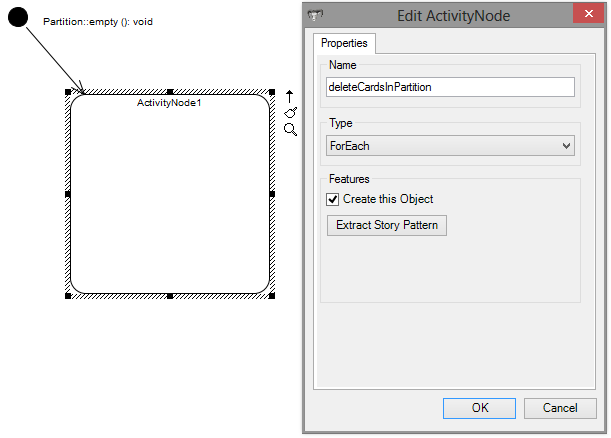
\includegraphics[width=0.9\textwidth]{ea_forEach}
  \caption{A for each loop in SDM.}  
  \label{fig:sdm_foreach}
\end{center}
\end{figure}

\vspace{1cm}

\item[$\blacktriangleright$] Next, complete the story pattern as indicated in Fig.~\ref{fig:sdm_end}. Please note that the \texttt{card} that is deleted in each match
is unbound, and both the \texttt{card} and link to \texttt{this} are set to \texttt{destroy}. Even more important, notice that the guard that terminates the for
each story node has an \texttt{[end]} guard. Indeed, a \emph{for each} story node \emph{must} have an end activity edge which is taken when all matches for the
story pattern have been handled.

\pagebreak

\begin{figure}[htbp]
\begin{center}
  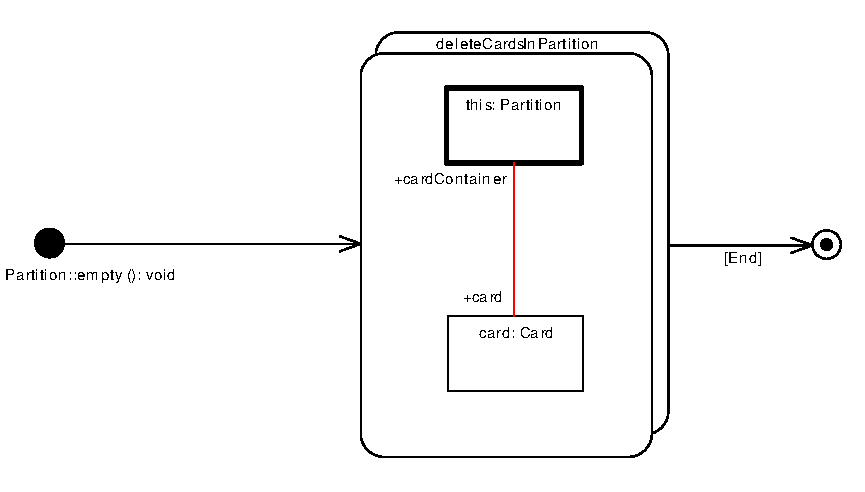
\includegraphics[width=0.9\textwidth]{ea_completeActivityEmptyCards.pdf}
  \caption{Complete story pattern with \texttt{[end]} guard.}  
  \label{fig:sdm_end}
\end{center}
\end{figure}

\fancyfoot[R]{ $\triangleright$ \hyperlink{sec:invertCard}{Next SDM} } \item[$\blacktriangleright$] Done! That's all we needed to do to specify a repeating
action. Pretty simple, eh? Inspect Figs. \ref{fig:emptyControlFlow} and \ref{fig:emptyPattern} to see how this is implemented textually.

\end{itemize}

